\documentclass[a4paper, 12pt]{article}
\usepackage[utf8]{inputenc}
\usepackage{geometry}
\usepackage{polski}
\usepackage{graphicx}
\usepackage{float}
\usepackage{etoolbox,refcount}
\usepackage{multicol}

\newgeometry{left=2cm, right=2cm, bottom=2cm, top=1.5cm}

\begin{document}
	\begin{figure}[H]
		\centering
		\includegraphics[height=6cm, width=\textwidth]{./img/lena.png}
	\end{figure}
	\section{Cel ćwiczenia}
		Celem tego ćwiczenia jest zapoznanie się z zasadami programowania sterowników PLC na przykładzie realizacji algorytmu regulacyjnego PID IND na sterowniku GE FANUC VERSAMAX MICRO.
	\section{Opis stanowiska}
		Stanowisko składa się z dwóch głównych części: 
		\begin{itemize}
			\item Komputer PC z oprogramowaniem VERSAPRO 1.1 pozwalającym na programowanie sterownika PLC, połączony z nim przez łącze szeregowe RS232
			\item Sterownik PLC z zespołem przełączników cyfrowych 
		\end{itemize}
		\begin{figure}[H]
			\centering
			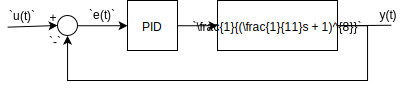
\includegraphics[height=6cm, width=\textwidth]{./img/schemat.png}
		\end{figure}
	\section{Wstęp}
		\subsection{Sterownik PLC}
			Sterowniki PLC są urządzeniami mikroprocesorowymi przeznaczonymi do sterowania pracą urządzenia technologicznego. Do działania sterownik PLC potrzebuje wgranego algorytmu dopasowanego do wymaganego zastosowania. Sterownik PLC posiada cykliczny obieg pamięci programu - po zakończeniu działania algorytm jest przeprowadzany od nowa.
			\newline 
			\newline
			Metody programowania są opisywane normą IEC 61131-3. W tym ćwiczeniu do programowania sterownika PLC używaliśmy logiki drabinkowej. Wiele programów zaprojektowanych do programowania sterowników PLC posiada również możliwość podglądu wykonywanego algorytmu.
		\subsection{Algorytm PID}
			Ze względu na cyfrową naturę sterowników PLC, mamy tu do czynienia z dyskretnym algorytmem PID. Ponieważ algorytm PID operuje w pętli sprzężenia zwrotnego, na wejściu podany jest uchyb, a na wyjściu znajduje się sterowanie wyprowadzone do układu. Dyskretne algorytmy PID dzielimy ze względu na:
			\begin{itemize}
				\item formę realizacji:
					\begin{itemize}
						\item pozycyjna -- mamy do czynienia z pełnymi wartościami
							$$
								u_n = ke_{n-1} + \frac{kT_p}{T_i} \sum_{i=0}^{n-1}e_i + kT_d \frac{e_{n-1} - e_{n-2}}{T_p}
							$$
							Wadą tej formy algorytmu jest łatwość w przepełnieniu części całkującej, co prowadzi do zakłamania sterowania. Zaletą natomiast jest możliwość realizacji wszystkich wersji algorytmu - P, PI, PD, PID.
						\item przyrostowa -- mamy do czynienia z przyrostami, jest to różnica kolejnych dwóch kroków algorytmu pozycyjnego
							$$
								\Delta u = k \Delta e_{n-1} + \frac{kT_p}{T_i} e_{n-1} + \frac{kT_d}{T_p} \Delta^2e_{n-1}
							$$
							gdzie:
							$$
								\Delta u_n = u_n - u_{n-1}
							$$
							$$
								\Delta e_{n-1} = e_{n-1} - e_{n-2}
							$$
							$$
								\Delta^2e_{n-1} = e_{n-1} - 2e_{n-2} + e_{n-3}
							$$
							Dużą przewagą tej realizacji algorytmu jest zmniejszenie szans na przepełnienie bufora całkowania. Wadą tego rozwiązania jest konieczność występowania członu całkującego w każdym z algorytmów, więc można przeprowadzić tylko regulację PI oraz PID. Dzieje się tak, gdyż w pozostałych przypadkach tracimy informację na temat wartości zadanej na skutek takiej samej liczby dodań jak i odejmowań uchybu\linebreak w wyznaczaniu każdej różnicy.
							
					\end{itemize}
				\item dobór parametrów:
					\begin{itemize}
						\item IND (INDependent algorithm) -- wszystkie współczynniki są niezależne od siebie, algorytm PID wygląda wtedy następująco:
							$$
								u_n = K_pe_{n-1} + K_iT_p \sum_{i=0}^{n-1}e_i + K_d \frac{e_{n-1} - e_{n-2}}{T_p}
							$$						
						\item ISA (Ideal Standard Algorithm) -- współczynniki są podane jako czas wyprzedzenia $T_d$, czas zdwojenia $T_i$ oraz wzmocnienie k:
							$$
								u_n = k\left(e_{n-1} + \frac{T_p}{T_i} \sum_{i=0}^{n-1}e_i + T_d \frac{e_{n-1} - e_{n-2}}{T_p}\right)
							$$	
					\end{itemize}
			\end{itemize}
			
	\section{Wykonanie ćwiczenia}
		Ćwiczenie rozpoczęliśmy od zbudowania układu, który pozwoliłby nam na przeprowadzenie algorytmu PID oraz na zamianę sygnału cyfrowego pochodzącego od przełączników na sygnał skoku jednostkowego. W celu tego wybraliśmy blok realizujący algorytm PID IND, gdyż o wiele wygodniej byłoby móc zmieniać poszczególne parametry algorytmu niezależnie od siebie (mimo tego, że w treści były podane przykładowe nastawy dla regulatora PID ISA).
		\begin{figure}[H]
			\centering
			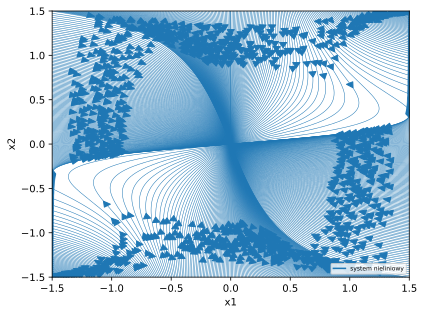
\includegraphics[width=0.7\textwidth]{./img/first.png}
		\end{figure}
		Podłączenia regulatora PID IND
		\begin{figure}[H]
			\centering
			\includegraphics[width=0.7\textwidth]{./img/second.png}
		\end{figure}
		Dzięki takiemu podłączeniu mogliśmy sterować zarówno ręcznie, jak i korzystając z regulatora PID. Po zaprogramowaniu układu zgraliśmy algorytm na sterownik PLC i uruchomiliśmy go dla różnych nastaw.
	\section{Przykładowy przebieg}
		\begin{figure}[H]
			\centering
			\includegraphics[]{./img/bonzo.png}
		\end{figure}
	\section{Wnioski}
		Ćwiczenie te pozwoliło nam na zapoznanie się z funkcjami oraz blokami funkcyjnymi oraz\linebreak z różnicą między nimi w logice drabinkowej, jak i nauczyło nas korzystać z logiki drabinkowej na oprogramowaniu VERSAPRO 1.1. Opanowaliśmy przy tym podstawy programowania sterowników PLC, które są obecnie często używane w różnego rodzaju układach automatyki ze względu na możliwości jakie udostępniają osobie programującej (chociażby bezpośredni dostęp do adresów pamięci) oraz ze względu na swoją wytrzymałość, która znaczenie przerasta tę zwykłych komputerów. 
		\newline
		\newline
		Język drabinkowy jest wygodny w użyciu, jeżeli chodzi o programowanie sterowników PLC, gdyż pozwala na zachowanie intuicji jaką się posiada z projektowania układów elektronicznych, pozwalając jednocześnie na pełne zastosowanie analogii do przepływu wody przez zawory. Jest to język przyjazny dla oka i prosty w debugowaniu ze względu na możliwość prostego podziału programu na mniejsze moduły, z których każdy zajmuje się czymś innym. Pomimo tylu zalet język ten może jednak sprawiać problemy dla osób, które znaczną część swojej przygody z programowaniem spędziły pisząc kod.
		\newline
		\newline
		Zapoznaliśmy się z blokiem funkcyjnym PID. Blok tren posiada sześć wejść: Enable (zezwól), Setpoint (wartość zadana), Process Variable (zmienna procesu), Man (sterowanie ręczne), Up Down oraz dwa wyjścia: OK, Control Variable. Zapoznaliśmy się tym samym z jednymi z najważniejszych pojęć automatyki w języku angielskim, w którym udostępniana jest znaczna część dokumentacji do wszelkiego rodzaju rozwiązań technologicznych.
		\newline
		\newline
		Oprogramowanie z którym mieliśmy do czynienia pozwalało nam na podgląd realizacji sterowania, co pozwalało nam szybko weryfikować błędne połączenia i je naprawiać, a podświetlanie poszczególnych podzespołów i wyświetlanie wyjść ze wszystkich bloczków użytych znacznie ułatwiło debugowanie połączeń oraz pozwoliło nam na intuicyjne śledzenie rejestrów wraz\linebreak z cewkami oraz stykami.
		\newline 
		\newline
		Wynieśliśmy z tego laboratorium teoretyczną wiedzę na temat dyskretnej realizacji algorytmu PID w różnych jego wersjach oraz wiedzę praktyczną z jego implementacji w logice drabinkowej wraz ze sprzężeniem zwrotnym. Mechanizm rejestrów i mechanizm cyklicznego obiegu pamięci programu znacznie nam to ułatwił, gdyż pozwalało nam to na zapisywanie wartości w jednym cyklu pracy i odczytywaniu jej przez maszynę na wejściu w następnym.
		\newline 
		\newline
		Nauczyliśmy się bardziej restrykcyjnego zarządzania pamięcią niż mamy z tym do czynienia\linebreak w wysokopoziomowych językach programowania lub też niskopoziomowych ograniczonych przez system operacyjny. W przypadku projektowania algorytmów na kontrolerach PLC nie mamy wygody korzystania z mechanizmów ochrony pamięci, przez co można bardzo łatwo nadpisać istotne dane, takie jak któryś z 40 kolejnych rejestrów wewnętrznych zajmowanych przez blok funkcyjny PID.
\end{document}